\documentclass{article}

\usepackage{graphicx}
\usepackage{tikz}
\usepackage{tikzsymbols}
\usetikzlibrary{calc,patterns,shapes.geometric}
\pagestyle{empty}
\usepackage[margin=0pt]{geometry}
\geometry{papersize={14in,12in}}

\def\centerarc[#1](#2)(#3:#4:#5){\draw[#1] ($(#2)+({#5*cos(#3)},{#5*sin(#3)})$) arc (#3:#4:#5);}

\begin{document}
	\begin{figure}
		\centering
		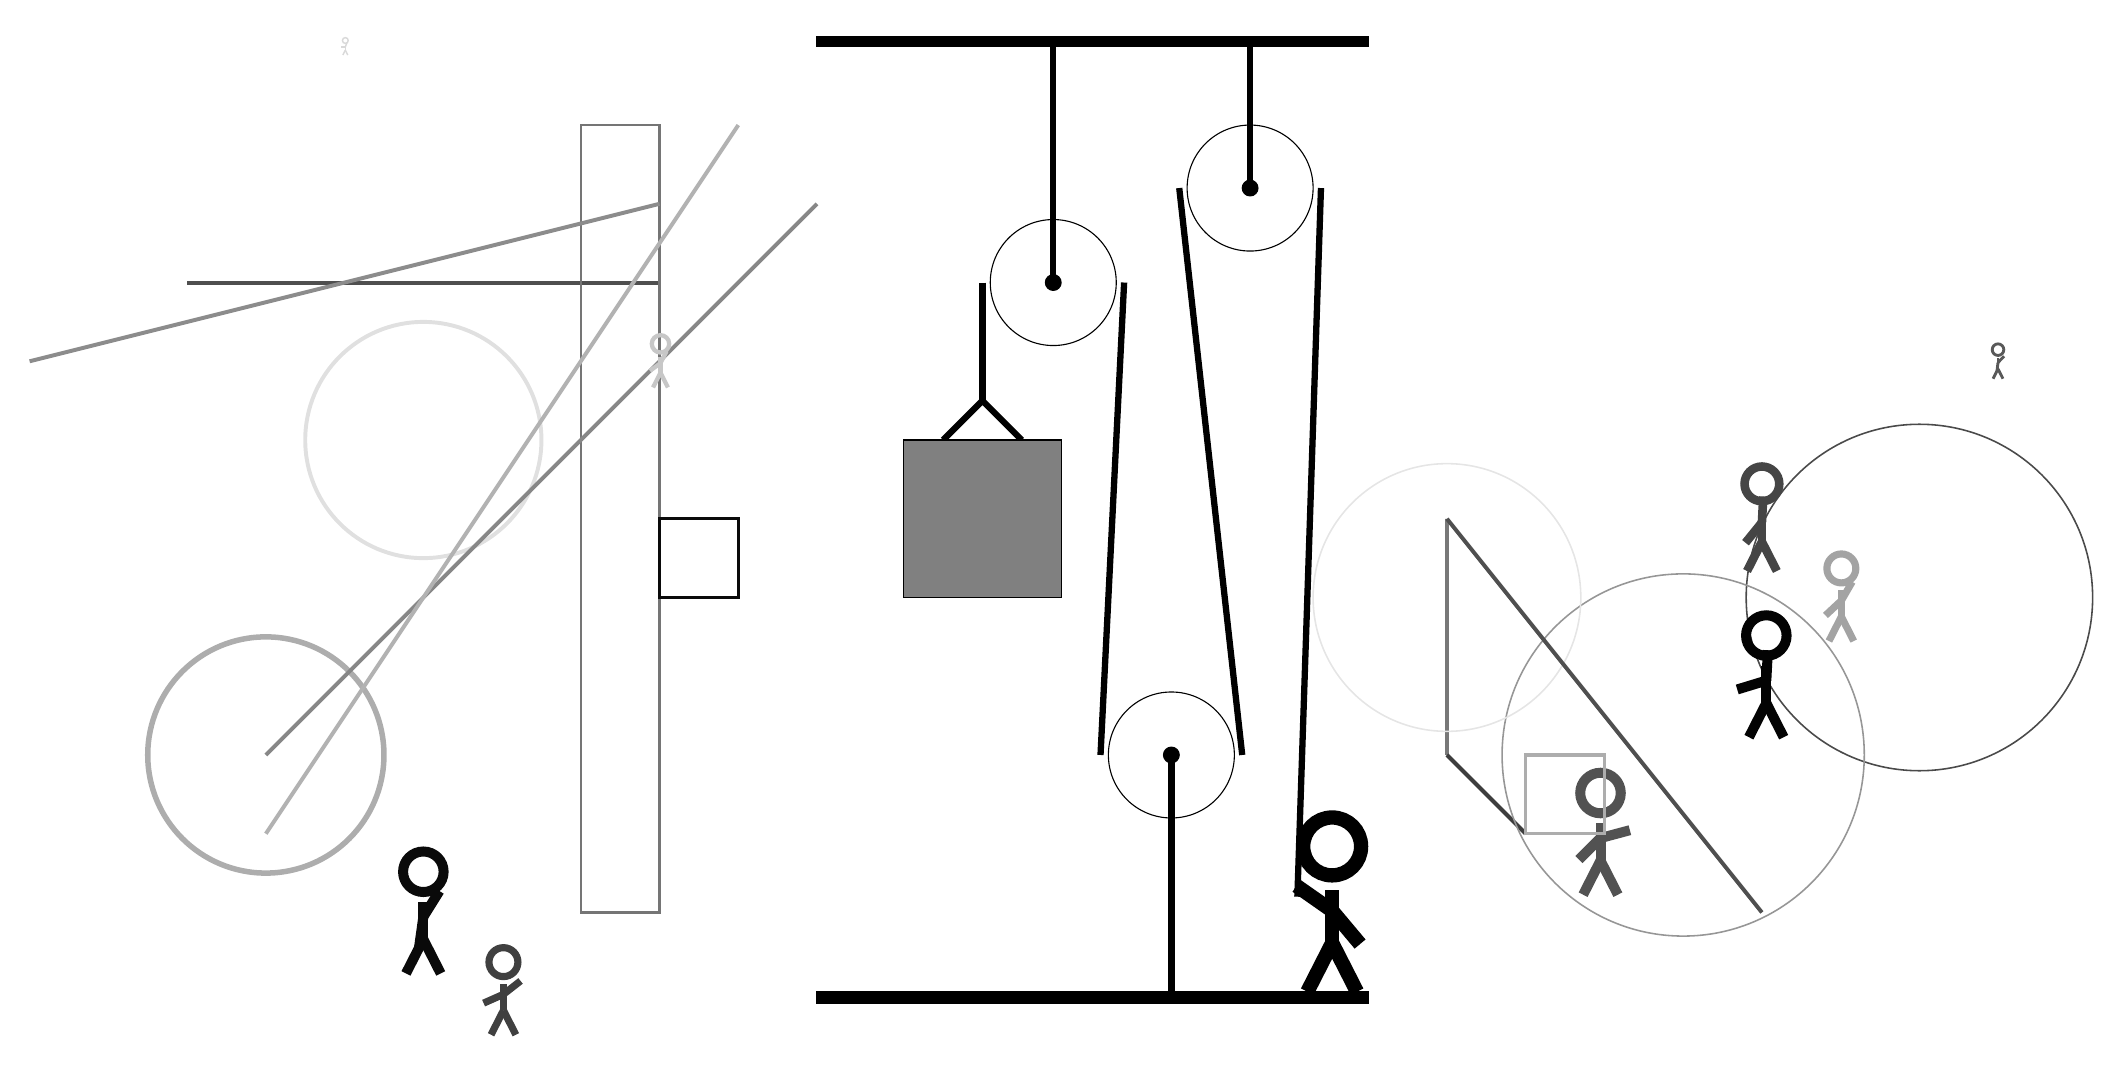
\begin{tikzpicture}
			%%%%% START %%%%%
			
			\draw[fill=black] (-2, 9) rectangle (5, 9.125);
			
			\draw (1, 6) circle (0.8);
			\draw[fill=black] (1, 6) circle (0.1);
			\draw[line width=0.8mm]  (1, 9) -- (1, 6);
			
			\draw[fill=white](2.5, 0) circle (0.8);
			\draw[fill=black] (2.5, 0) circle (0.1);
			\draw[line width=0.8mm]  (2.5, -3) -- (2.5, 0);
			
			\draw[fill=white](3.5, 7.2) circle (0.8);
			\draw[fill=black] (3.5, 7.2) circle (0.1);
			\draw[line width=0.8mm] (3.5, 9) -- (3.5, 7.2);
			
			\draw [line width=0.7mm, color=black!32](-9, 0) circle (1.5);
			
			\node[line width=0.2mm, color=black!15] at (-8, 9) {\Strichmaxerl[1][0][69]};
			\draw[line width=0.5mm, color=black!53] (6, 3) rectangle (6, 0);
			\draw [line width=0.2mm, color=black!71](12, 2) circle (2.2);
			\node[line width=0.7mm, color=black!75] at (-6, -3) {\Strichmaxerl[5][24][38]};
			
			\draw[line width=0.5mm, color=black!69](-4, 6) -- (-10, 6);
			\node[line width=0.2mm, color=black!68] at (8, -1) {\Strichmaxerl[7][45][15]};
			\draw[line width=0.3mm, color=black!54] (-4, 8) rectangle (-5, -2);
			\node[line width=0.6mm, color=black!36] at (11, 2) {\Strichmaxerl[5][43][60]};
			\draw [line width=0.5mm, color=black!12](-7, 4) circle (1.5);
			
			\draw[line width=0.5mm, color=black!47](-2, 7) -- (-9, 0);
			\draw[line width=0.5mm, color=black!76](7, -1) -- (6, 0);
			\draw [line width=0.2mm, color=black!41](9, 0) circle (2.3);
			\node[line width=0.4mm, color=black!99] at (10, 1) {\Strichmaxerl[7][17][87]};
			\draw[line width=0.5mm, color=black!45](-4, 7) -- (-12, 5);
			\node[line width=0.6mm, color=black!96] at (-7, -2) {\Strichmaxerl[7][82][58]};
			
			\draw[line width=0.4mm, color=black!32] (7, -1) rectangle (8, 0);
			
			\node[line width=0.7mm, color=black!22] at (-4, 5) {\Strichmaxerl[3][36][63]};
			\node[line width=0.6mm, color=black!65] at (13, 5) {\Strichmaxerl[2][83][46]};
			\draw [line width=0.2mm, color=black!10](6, 2) circle (1.7);
			\draw[line width=0.4mm, color=black!96] (-3, 3) rectangle (-4, 2);
			
			\draw[line width=0.5mm, color=black!69](6, 3) -- (10, -2);
			\draw[line width=0.5mm, color=black!30](-3, 8) -- (-9, -1);
			\node[line width=0.6mm, color=black!73] at (10, 3) {\Strichmaxerl[6][51][87]};
			
			\draw[line width=0.8mm] (-0.4, 4.0) -- (0.1, 4.5) -- (0.6, 4.0);
			\draw[fill=black!50] (-0.9, 4.0) rectangle (1.1, 2.0);
			
			\draw[line width=0.8mm] (0.1, 6) -- (0.1, 4.5);
			\centerarc[line width=0.8mm](1, 6)(0:180:0.9);
			\draw[line width=0.8mm](1.9, 6) -- (1.6, 0);
			\centerarc[line width=0.8mm](2.5, 0)(180:360:0.9);
			\draw[line width=0.8mm](3.4, 0) -- (2.6, 7.2);
			\centerarc[line width=0.8mm](3.5, 7.2)(0:180:0.9);
			\draw[line width=0.8mm](4.4, 7.2) -- (4.1, -1.8);
			
			\node at (4.5, -1.9) {\Strichmaxerl[10][-35][-50]};
			
			\draw[fill=black] (-2, -3) rectangle (5, -3.15);
			
			%%%%% END %%%%%
		\end{tikzpicture}
	\end{figure}	
\end{document}